\documentclass[a4paper, 11pt, ngerman, fleqn]{article}
\usepackage[utf8]{inputenc}
\usepackage[ngerman, english]{babel}
\usepackage{coordsys,logsys,color}
\usepackage{hyperref}
\usepackage{texdraw}
\usepackage{fancyhdr}
\usepackage{graphicx}
\input{txdtools}

\NeedsTeXFormat{LaTeX2e}
\ProvidesPackage{hyperref}
\definecolor{darkblue}{rgb}{0,0,.6}
\hypersetup{pdftex=false, colorlinks=true, breaklinks=true, linkcolor=darkblue, menucolor=darkblue, urlcolor=darkblue, citecolor=darkblue}

\pagestyle{fancy}

%\renewcommand{\familydefault}{cmss}

\definecolor{fgcgray}{rgb}{0.4, 0.4, 0.4}
\definecolor{warning}{rgb}{0.9, 0.1, 0.0}
\definecolor{bgctitle}{rgb}{0.5, 0.5, 0.5}
\definecolor{fgctitle}{rgb}{0.95, 0.95, 0.95}
\newcommand{\titlefont}[1]{\textcolor{fgctitle}{\fontfamily{cmss}\fontseries{bx}\fontshape{n}\fontsize{20.48}{0pt} \selectfont #1}}
\newcommand{\inversetitlefont}[1]{\textcolor{bgctitle}{\fontfamily{cmss}\fontseries{bx}\fontshape{n}\fontsize{20.48}{0pt} \selectfont #1}}

\addtolength{\oddsidemargin}{-1.0cm}
\addtolength{\evensidemargin}{-1.0cm}
\addtolength{\headwidth}{2.0cm}
\addtolength{\textwidth}{2.0cm}

\setlength{\parindent}{0cm}

\renewcommand{\labelitemi}{$\circ$}
\renewcommand{\labelitemii}{$\diamond$}

\newcommand{\spaceline}[1][8pt]{\vskip #1}
\newcommand{\comment}[1]{\spaceline[5pt] \textcolor{fgcgray}{\scriptsize #1} \spaceline[15pt]}
\newcommand{\attrname}[1]{\textcolor{fgcgray}{\scriptsize #1}}


\makeatletter

\newcommand*{\project}[1]{\gdef\@project{#1}}
\newcommand*{\version}[1]{\gdef\@version{#1}}
\newcommand*{\home}[1]{\gdef\@home{#1}}
\newcommand*{\homeref}[1]{\gdef\@homeref{#1}}

\def\@maketitle{
  %\begin{titlepage}
  \begin{center}
    \colorbox{bgctitle}{
      \parbox{\textwidth}{
        \spaceline
        \centering{\titlefont{\@title}}
        \par
        \spaceline
      }
    }
    \colorbox{white}{
      \parbox{\textwidth}{
        \spaceline
        \centering{\inversetitlefont{\@project}}
        \par
        \spaceline
      }
    }
  \end{center}
  \spaceline[1.5em] {
    \begin{flushright}
    \begin{tabular}[t]{rl}
      \attrname{Projekt:} & \@project ~ \@version \\
      \attrname{Autor:} & \@author \\
      \attrname{letzte "Anderung:} & \@date
    \end{tabular}
    \end{flushright}
    \par
  }
  \spaceline[5.5em]
  %\end{titlepage}
}

\setcounter{secnumdepth}{4}
\setcounter{tocdepth}{4}

\newcounter{subsubsubsection}[subsubsection]
\def\subsubsubsectionmark#1{}
\def\thesubsubsubsection{\thesubsubsection .\arabic{subsubsubsection}}
\def\subsubsubsection{\@startsection{subsubsubsection}{4}{\z@}{-3.25ex plus -1 ex minus -.2ex}{1.5ex plus .2ex}{\normalsize\bf}}
\def\l@subsubsubsection{\@dottedtocline{4}{4.8em}{4.2em}}

\makeatother

\everytexdraw{
  \drawdim cm \linewd 0.01
  \arrowheadtype t:T
  \arrowheadsize l:0.2 w:0.2
  \setgray 0.5
}

\newcommand{\xheight}{0.6}
\newcommand{\xlength}{0.6}
\newcommand{\yheighta}{1.0}
\newcommand{\yheightb}{0.8}
\newcommand{\yheightc}{0.6}
\newcommand{\yheightd}{0.5}
\newcommand{\yheighte}{0.4}
\newcommand{\yheightf}{0.35}

\newcommand{\xhline}{\rlvec({\xlength} 0)}
\newcommand{\xharrow}{\ravec(0.7 0)}
\newcommand{\xnext}{%\rlvec(0.05 0) \lpatt(0.04 0.04) \rlvec(0.15 0) \lpatt()
}

\newcommand{\xtext}[3][\xheight]{
  \bsegment
    \bsegment
      \setsegscale 0.5
      \textref h:L v:C  \htext({\xheight} -0.1){#3}
    \esegment
    \setsegscale 0.5 \lvec(0 #1)
    \setsegscale 1
    \rlvec(#2 0) \rlvec(0 -#1) \rlvec(-#2 0) \lvec(0 0)
    \savepos(#2 0)(*@x *@y)
  \esegment
  \move(*@x *@y)
}

\newcommand{\bxtext}[3][\xheight]{
  \setgray{0.1}
  \linewd{0.026}
  \xtext[\xheight]{#2}{#3}
  \linewd{0.01}
  \setgray{0.5}
}

\newcommand{\xstartpage}{\bxtext{2.1}{Startseite}}
\newcommand{\xmainpage}{\bxtext{2.3}{Hauptseite}}
\newcommand{\xusermenu}{\bxtext{2.9}{Benutzermenu}}
\newcommand{\xgamelist}{\bxtext{2.2}{Spieleliste}}
\newcommand{\xportfolio}{\bxtext{2.0}{Portfolio}}
\newcommand{\xaccount}{\xtext{3.8}{Kennung per \textsl{eMail}}}


\begin{document}
  \lhead{\sc{Virtual Reality for Sensor Data Analysis}}
%\cfoot{-~\thepage~-}
\title{Pflichtenheft}
\project{Virtual Reality for Sensor Data Analysis}
\version{0.1}
\author{Gero Birkhölzer, Johannes Blank, Alexej Gluschkow, Fabian Klopfer, Lisa-Maria Mayer}
\maketitle
%\thispagestyle{empty}
%~
%\newpage
%\tableofcontents
 \newpage
  \tableofcontents \newpage
  \section{Purpose}
The software project module in 2017 at the University of Constance focuses on the development of an app for mobile devices. \\
Especially, this Pflichtenheft intends to describe the structure of an implementation of a virtual reality representation of BLE sensor feedback.

\subsection{Mandatory Criteria}

\begin{description}
  \item[M1] The app shall use the Bluetooth adapter of the smartphone to connect to a TI SimpleLink SensorTag device.
  \item[M2] The app shall track the position of a TI SimpleLink SensorTag device with up to 30m tolerance.
  \item[M3] The app shall visualize the sensors' data and its position using 3D/stereoscopy, more concrete the WebVR framework.
  \item[M4] The visualization mentioned in M3 shall be explorable by tilting the joystick of a bluetooth controller.
  \item[M5] The VR-World shall represent at least two different rooms and a connecting hallway.
  \item[M7] The data from the sensor shall have two different representations in the VR-World.
  \item[M8] The app shall provide a live data view of the sensor feedback in human readable form.

\end{description}

\subsection{Desired Criteria}

\begin{description}
  \item[A1] The app shall visualize the sensors' data and its position using augmented reality.
  \item[A2] The VR-World shall represent a whole corridor with more than two rooms.
  \item[A3] The app shall store the sensors' data and give a time lapse of the data inside the VR-World.
\end{description}
 \newpage
  \section{Product Environment}

\subsection{Software}

\begin{itemize}
  \item Android 5.0 Lollipop or higher
\end{itemize}

\subsection{Hardware}

\begin{itemize}
  \item Bluetooth-enabled Smartphone
  \item TI SimpleLink SensorTag device
  \item Victorstar VRBox 2.0
  \item VR-Park Bluetooth Controller
\end{itemize}
 \newpage
  \section{Product Functions}

%\comment{functional Requirements}

\subsection{Settings}
  The User can set the following Options:
  \begin{description}
    \item[/F0100/]
  	\textit{Sensor:} The User can set, which data shall be displayed in the VR-World (Temperature, etc.)
  \end{description}

\subsection{VR-World}
  The VR-Mode is 3D view of the world on entering VR-Mode the user will see a fullscreen 3D world and by pressing the button in the lower right corner he can enter the  stereoscopic view of the World.
  The VR-World is a 3D representation of a real series of rooms.
  \begin{description}
    \item[/F0300/]
      \textit{Look around:} The User can look around in the Vr-World by touching and draging on the Screen or by moving his head around to pan the camera.
  \end{description}

  \begin{description}
    \item[/F0310/]

      \textit{Move inside VR-World:} The User can move inside the VR-World by tilting the joystick of his controller forward. Turning will be done by looking around with the VR-headset
                                    or by clicking and dragging on the screen.
  \end{description}

  \begin{description}
    \item[/F0320/]
      \textit{Switch Data representation:} The User can switch between two different respresentations of the bluetooth data from the sensor by pressing the A-Button on his controller.
  \end{description}

  \begin{description}
    \item[/F0330/]
      \textit{Exit VR-Mode:} The User can exit the VR-Mode by pressing the x in the top right corner of the screen or by looking for 5 seconds directly on the x under his feet.
  \end{description}

  \begin{description}
    \item[/F0340/]
  	\textit{Enter stereoscopic VR-Mode:} The User can switch from fullscreen VR-Mode to stereoscopic by pressing the button in the lower right corner or by pressing the A-Button on his controller.
  \end{description}

  \begin{description}
    \item[/F0350/]
      \textit{Exit stereoscopic VR-Mode:} The User can leave stereoscopic Vr-Mode by pressing the back button on his device or by touching the back button in the top left corner.
  \end{description}

  \begin{description}
    \item[/F0360/]
      \textit{Enter Settings:} The User shall be able to enter the Settings menu while in normal 3D-Mode.
  \end{description}

  \begin{description}
    \item[/F0370/]
      \textit{Switch rooms:} The User can easily switch rooms by pressing the B-Button on his controller or by looking up at the door sign for at least 5 seconds.
  \end{description}

  \begin{description}
    \item The VR-World shall model at least two different rooms and a connect hallway.
    \item The VR-World shall be viewed inside a web browser and from the App.
    \item The VR-World shall have a stereoscopic 3D-Mode of the World.
    \item While viewing the VR-World the user shall be able to look around using the gyro senor of his phone to pan the camera around.
    \item While the App is not in stereoscopic 3D mode the User shall be able to click and drag to pan the camera around.
    \item The User shall be able to move the camera inside the Vr-World by using his controller.
    \item The Data fechted from the Sensor shall be displayed inside the VR-World.
    \item There shall be at least two different representations the data from the Sensor.
    \item The VR-World shall represent at least two different real world rooms.
    \item The User shall be able to easily switch between stereoscopic 3D and normal 3D mode.
    \item The App shall be in fullscreen mode, while in VR-Mode.
    \item While in stereoscopic 3D-Mode the user shall be able to exit it by looking for 5 seconds at the cross under his feet.
  \end{description}
 \newpage
  \section{Proposed Architecture}

\subsection{Overview}

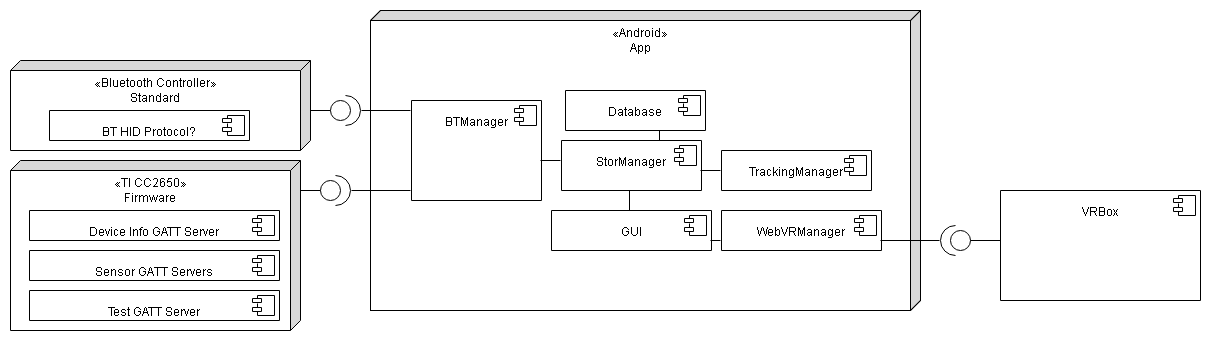
\includegraphics[scale=0.35]{pics/composite_app.png}

\subsection{Component Decomposition}

\subsubsection{Services}
From \href{https://developer.android.com/guide/components/services.html}{AndroidDoc}: \\
``A Service is an application component that can perform long-running operations in the background, and it does not provide a user interface''.
\begin{itemize}
  \item \textbf{BluetoothManager:} Uses the android.bluetooth and especially the android.bluetooth.le libraries to fetch the sensor data from the TI CC2650.
  \item \textbf{TrackingManager:} Handles the tracking of the cellphone and therefore of the TI SensorTag devices. the current position gets determined by GPS and enhanced by the cellphone sensor and wifi data.
  \begin{center}
  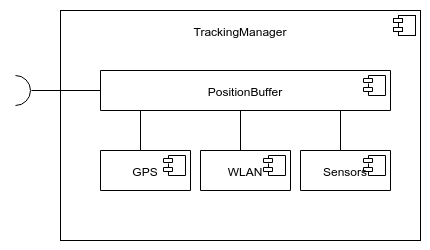
\includegraphics[scale=0.4]{pics/TrackingManager_Composition.png}
  \end{center}
  
  \item \textbf{WebVRManager:} Uses webview to display the WebVr-World and communicates with the WebVr-Site.
  \item \textbf{StorageManager:} uses a DB (z.B. NeDB or internal stor or similar to safe parsed sensor input, location, settings,...)
  \item \textbf{VRBox:} Handles the display of the Vr-World and the given data from the sensor.

  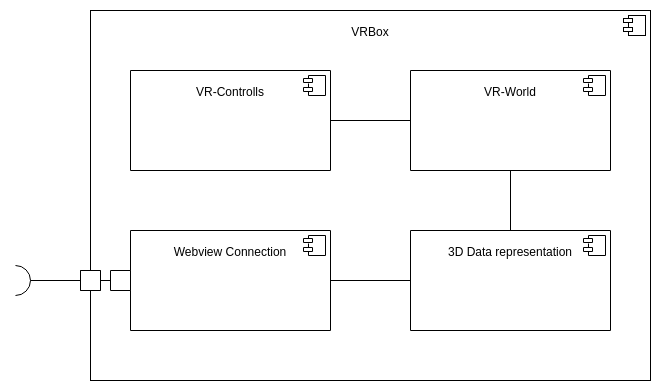
\includegraphics[scale=0.35]{pics/VRBox.png}

\end{itemize}


\subsubsection{GUI}
From \href{https://developer.android.com/guide/components/services.html}{AndroidDoc}: \\
``They (Activities) serve as the entry point for a user's interaction with an app, and are also central to how a user navigates within an app (as with the Back button) or between apps (as with the Recents button)''. \newline
\begin{itemize}
  \item \textbf{MainActivity} Provides the main startup screen as the main entry point.
  \item \textbf{VRViewActivity} shall provide the WebVR view using the android.webkit library (especially .webview).
  \item \textbf{LiveDataActivity} shall provide a view of the sensor data in human readable form.
  \item \textbf{TISettingsActivity:} Settings screen containing scanning and connecting, connected devices and device settings fragments.
  \begin{itemize}
    \item \textbf{ScanningConnectingFragment} shall show the scanning results, delivered by the SensorTagBluetoothReceiverService and controll to which device to connect to or disconnect.
    \item \textbf{ConnectedDevicesFragment} shall show a list of all connected devices and a short info about the current setting and state of the TI SimpleLink SensorTag device.
    \item \textbf{ConnectedDevicesSettingsFragment} shall implement the configuration of the app features of the sensor.
  \end{itemize}
\end{itemize}

\subsubsection{Additional Classes}
\begin{itemize}
  \item \textbf{GATT Profiles} (for each sensor one)
  \item \textbf{GATT Sensor Service UUIDs}
  \item \textbf{Parser Functions} because the BLE protocol implemented in the TI CC2650 delivers raw sensor output
\end{itemize}
 \newpage
  \section{Product Data}

\subsection{VR-World}

\begin{description}
  \item[D1.1] \textbf{Models:} The modeles used to render the VR-World will be saved as .obj files using Blender in /webvr/models/.
  \item[D1.2] \textbf{Textures:} As .png files in /webvr/img/.
\end{description}
%TODO: MockUp/Interface einer Projekt 4 Gruppe \\
%TODO: Was muss für 3D Modell gespeichert werden? Wie sehen die Datenstrukturen aus? \\

%Jeder Punkt \textbf{/D???/} stellt im Prinzip einen Datensatz dar.

%\begin{description}
%  \item[/D010/]
%    \textit{Benutzerdaten:} Alle Informationen zu einem Benutzer:
%    \begin{itemize}
%      \item \textbf{BenutzerID} \textit{(eindeutig)}
%      \item Kennung
%        \begin{itemize}
%          \item \textbf{Benutzername} \textit{(eindeutig)}
%          \item \textbf{Passwort} \textit{(verschlüsselt)}
%        \end{itemize}
%    \end{itemize}
%\end{description}
 \newpage
  \section{User interface}

\subsection{Structure}

A small overview of the menu Structure.

\subsubsection{Start screen}

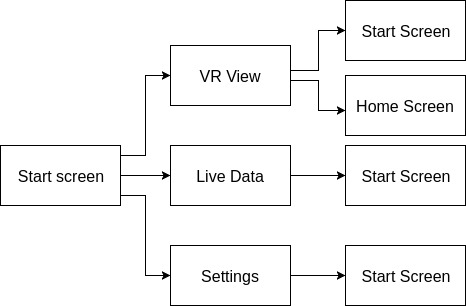
\includegraphics[scale=0.5]{pics/startscreen.jpg}

\subsubsection{VR-Mode}

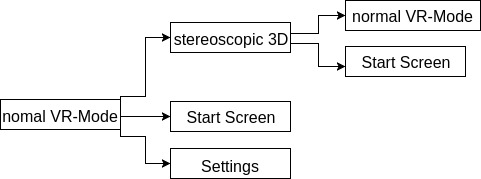
\includegraphics[scale=0.5]{pics/Vr-Mode.jpg}


\subsubsection{Live Data}

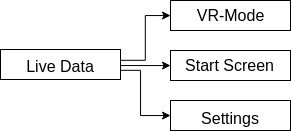
\includegraphics[scale=0.5]{pics/Live_Data.jpg}

\subsubsection{Settings}

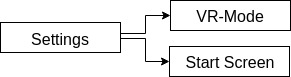
\includegraphics[scale=0.5]{pics/Settings.jpg}

\newpage
\subsection{Layout}

A mockup of the Start up screen.
\\
\\
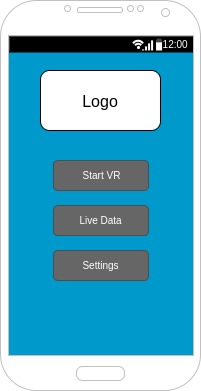
\includegraphics[scale=0.5]{pics/startScreen_mockup.jpg}
\\

And a mockup of the stereoscopic Vr-Mode.
\\
\\
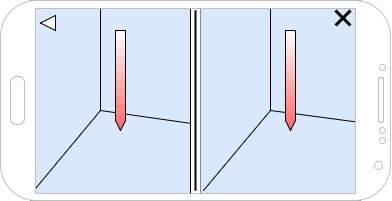
\includegraphics[scale=0.5]{pics/VRView_mockup.jpg}
 \newpage
  \section{Quality Requirements}

%\comment{Auf welche Qualitätsanforderungen (Zuverlässigkeit, Robustheit, Benutzungsfreundlichkeit, Effizienz, ...) wird besonderen Wert gelegt?}

\begin{center}
 \begin{tabular}{l|c|c|c|c}
  ~ & very important & important & less important & lesser important \\
  \hline \hline
  \textit{Robustness}~ &  ~ ~ ~ &  ~ ~ ~ &  ~ ~ ~ & \textbf{X}~ \\
  \hline
  \textit{Reliability}~ & \textbf{X}~ &  ~ ~ ~ &  ~ ~ ~ &  ~ ~ ~ \\
  \hline
  \textit{Correctness}~ & \textbf{X}~ &  ~ ~ ~ &  ~ ~ ~ &  ~ ~ ~ \\
  \hline
  \textit{Usability}~ & \textbf{X}~ & ~ ~ ~ &  ~ ~ ~ &  ~ ~ ~ \\
  \hline
  \textit{Efficiency}~ &  ~ ~ ~ & \textbf{X}~ &  ~ ~ ~ &  ~ ~ ~ \\
  \hline
  \textit{Portability}~ &  ~ ~ ~ & \textbf{X}~ &  ~ ~ ~ &  ~ ~ ~ \\
  \hline
  \textit{Compatibility}~ &  ~ ~ ~ &  ~ ~ ~ & \textbf{X}~ &  ~ ~ ~ \\
 \end{tabular}
\end{center}
 \newpage
  \section{Test Cases}

%\comment{Was sind typische Szenarien, die das Produkt erfüllen muss?}
%\comment{tests für alle requirements; am ende}

%Jede Produktfunktion \textit{/F????/} wird anhand von konkreten Testfällen \textit{/T????/} getestet.\\
%Die dabei verwendeten Namen werden rein zufällig gewählt.

%\begin{description}
%  \item[/T????/]
%    ...
%\end{description}


\begin{description}
  \item[/T0300/]
    \textit{Look around:} While in normal 3D mode the tester shall click the screen and drag first up to move the camera up.
    Then move down to move the camera down, then at last left and then right, all the time the camera must follow the movement of the finger.
    After this the tester shall tilt the phone up to move the camera up, then tilt it down, left and right. The camera shall follow the tilt direction of the phone all the time with no delay.

    This test will be repeated in stereoscopic 3D view, while the clicking and dragging shall not work, the tilting of the phone shall be the only way to pan the camera.
\end{description}

\begin{description}
  \item[/T0310]
    \textit{Move inside VR-World:} While in nomral 3D mode the Tester shall tilt the joystick on the conrtoller forward and the camera shall move forward.
    By tilting the joystick backward the camera shall move back, by tilting left the camera shall move left and by tilting right it shall move right.
    The camera shall allways follow the view point, so forward is allways in the center of the camera.

    This test shall be again repeated in stereoscopic 3D view and all funcitons shall work the same.
\end{description}
 \newpage
  \section{Development Environment}

\subsection{Software}

\begin{itemize}
  \item[OS] Windows 10, macOS Sierra
  \item[IDEs]  Android Studio, Sensor Controller Studio 1.4.1
  \item[VCS] Git,GitHub
  \item[UML-Editor] Enterprise Architekt, MS Visio, \href{draw.io}{draw.io}
  \item[Zeichensatz] \LaTeX

\end{itemize}

\subsection{Hardware}

\begin{itemize}
  \item[Smartphone] Motorola XT1572
  \item[Sensor] TI CC2650STK
  \item[VR-Headset] Victorstar VRBox 2.0
  \item[Bluetooth-Controller] VR-Park (?)
\end{itemize}
 \newpage
  \section{Project Time Line}


\begin{tabular}{l|p{12cm}}

\textbf{Week / Final Date}  & \textbf{Event / Tasks} \\ \hline

\textbf{25.5.- 1.5.} & first research, write Pflichtenheft \\ 
2.5. & release Pflichtenheft, project plan, subjects of milestones\\ \hline
\textbf{2.5.- 8.5.} & distribute tasks, decide on design\\ 
\textbf{9.5.- 15.5.} & start building \\ 
\textbf{16.5.- 22.5.} & \\
22.5. & \textit{Milestone 1:} Basic functions are implemented (gathering data, display data in app, build a basic 3D world) \\ \hline
\textbf{23.5.- 29.5.} &  \\
\textbf{30.5.- 5.6.} & \\
\textbf{6.6.- 12.6.} & \\
12.6. & \textit{Milestone 2:} Gathered data can be displayed in 3D, \textit{intermediate assessment} \\ \hline
\textbf{13.6.- 19.6.} & \\
\textbf{20.6.- 26.6.} & \\
\textbf{27.6.- 3.7.} & \\
\textbf{4.7.- 10.7.} & \\
\textbf{11.7.- 17.7.} & \\
17.7. & \textit{Milestone 3:} The app works as wanted :D \\ \hline
\textbf{18.7.- 24.7.} & prepare presentation and usage examples\\
25.7. & \textit{final presentation }

\end{tabular} \\



Possible starting points: \\
\href{https://bitbucket.org/StylingAndroid/bluetoothle/src/1fe191cf34f34f9917b1d0d62c617c607fe3df4d/src/main/java/com/stylingandroid/ble/?at=Part2}{Simple, bad layout} \\
\href{https://git.ti.com/sensortag-20-android/sensortag-20-android/trees/master/sensortag20/BleSensorTag/src/main/java/com/example/ti}{TI official, complex}
 \newpage
\end{document}
